\documentclass{article}
\usepackage[shortlabels]{enumitem}
\usepackage{amsmath}
\usepackage{graphicx}
\usepackage{placeins}
\usepackage{caption}
\usepackage[procnames]{listings}
\usepackage{color}
\usepackage{subcaption}
\usepackage{amsthm}

\begin{document}
% All of this is for highlighting of Python code
\definecolor{keywords}{RGB}{255,0,90}
\definecolor{comments}{RGB}{0,0,113}
\definecolor{red}{RGB}{160,0,0}
\definecolor{green}{RGB}{0,150,0}
 
\lstset{language=Python, 
        basicstyle=\ttfamily\small, 
        keywordstyle=\color{keywords},
        commentstyle=\color{comments},
        stringstyle=\color{red},
        showstringspaces=false,
        identifierstyle=\color{green},
        procnamekeys={def,class}}



\title{Image Feature Analysis}
\author{Nicolas Langley 904433991}
\maketitle
\section{Introduction}

This project looks to perform analysis of image characteristics using a Convolutional
Neural Network in order to identify specific image features.  

\section{Dataset Overview}

An overview of the datasets used in this project will be presented as follows:
\begin{enumerate}
  \item Dataset Contents
  \item Dataset Origins
  \item Relevance to Project
\end{enumerate}

\subsection{MNIST Dataset}

\begin{enumerate}
  \item The MNIST dataset contains a large number of handwritten digits. It contains 50,000 training
        examples as well as 10,000 testing samples. Each of the samples is a single handwritten digit
        from 0 to 9 centered in a $28x28$ image. This centering is done by computing the center of mass
        of the pixels in the data and translating the image so this point is at the center of the $28x28$
        image. 
  \item The dataset is a subset of the a database compiled by the National Institute of Standards and Technology
        (NIST) comprised of handwritten digits by both Census Bureau Employees and High School students. The MNIST 
        dataset is a re-mixed subset where half of the training images and half of the testing images were taken 
        from each of the Census Bureau Employee and High School student sets respectively.
  \item This dataset is very commonly used as an initial dataset for the testing of different machine learning
        techniques. For this project, it was used as the initial dataset for testing the implementation of the
        convolutional neural network (CNN) approach used. It was also used in the testing of the PCA-based technique.
        For the purpose of working with the CNN, the training dataset was divided into both a training and a validation
        data set
        \FloatBarrier
        \begin{figure}
          \caption{Sample of the MNIST dataset}
          \centering
          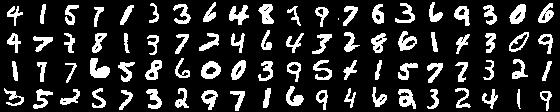
\includegraphics[scale=0.5]{images/mnist_dataset_example}
        \end{figure}
        \FloatBarrier
\end{enumerate}

\subsection{CIFAR Dataset}

\begin{enumerate}
  \item The CIFAR datasets are two datasets that contain a set of labelled $32x32$ color images. There are two
        versions of the dataset: one where the images are divided into 10 classes (CIFAR-10) and one where they are divided
        into 100 different classes (CIFAR-100). For this project, the CIFAR-100 dataset was used with a focus of the "coarse"
        labels provided (there are 20 coarse labels and 100 fine labels)
  \item These datasets are labelled subsets of the Tiny Images Dataset. The Tiny Images Dataset is a dataset of 80 million
        different $32x32$ images. The CIFAR datasets are comprised of a sampling of these images where the chosen images have
        been divided into classes and labelled.
  \item Within the context of this project, the CIFAR dataset was used as input to the Convolutional Neural Network as a more complex
        dataset than the MNIST dataset with real world (useful) classes that could be used in the identification process. A copy of the
        dataset was constructed where the images have been simplified by reducing their size to $28x28$ and converted to grayscale images.
        The images have also been whitened using PCA
        \FloatBarrier
        \begin{figure}[h]
          \centering
          \begin{subfigure}{\textwidth}
            \centering
            \caption{Sample of original CIFAR dataset}
            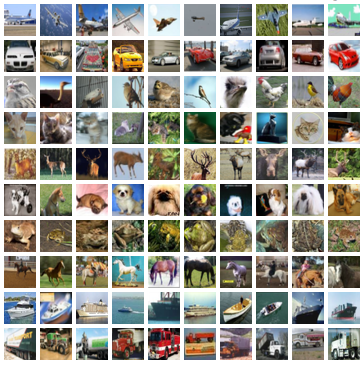
\includegraphics[scale=0.4]{images/cifar_dataset_example}
          \end{subfigure}
        \end{figure}
        \FloatBarrier
\end{enumerate}

\subsection{Custom Dataset}

\begin{enumerate}
  \item Test
\end{enumerate}

\newpage
\section{Overview of Techniques}

This project involved the exploration of a number of techniques used to determine the features of an image. The technique that was settled
on and used for the attempted gathering of results was the Convolutional Neural Network. Other explored results were the use of Principal
Components Analysis on a set of images as well as simple MultiLayer Perceptrons and Logistic Regression. This report will go into detail on
the approach taken for testing each of these techniques as well as their results with respect to the goal of the project.

\subsection{Principal Components Analysis and Whitening}
  \subsubsection{Technique Overview}
  
  Principal Components Analysis (PCA) is a technique for converting a set of correlated variables into a set of linearly uncorrelated variables
  called Principal Components. The Principal Components are orthogonal to each other and starting with the first Principal Component, represent
  (in decreasing order) the largest possible variance. These Principal Components can be found by taking the eigendecomposition of the covariance
  matrix of a set of data. The Principal Components correspond to the eigenvectors of this decomposition.

  In this project, PCA was initially used as an approach for extracting the features of an image. This approach involves looking at a large set of
  like-images and extracting the Principal Components. These Principal Components will represent the areas of highest variance within the image and
  can be interpreted as being the features of the image set.
  
  PCA was used in preparation of the image data used as a part of the Whitening Transformation. The Whitening Transformation is a decorrelation
  transformation that transforms a set of random variables with a covariance matrix, $M$ into a set of random variables with the Identity matrix as
  their covariance matrix. This transformation serves to change the input vector into a white noise vector where all the random variables are decorrelated
  and their variance is 1. This transformation involves the following steps: \\
  \begin{enumerate}
    \item Given a data matrix $X_{k,n}$, center the data by subtracting the mean.
	\item Compute the covariance matrix $\Sigma = X X^{T} / n$
	\item Take the Eigenvalue Decomposition of $\Sigma$ to be $\Sigma = E D E^{T}$
	\item Re-arrange to get $D = E^{T} \Sigma E$
	\item Multiply the data $X$ by $D^{-\frac{1}{2}} E^{T}$ to get the 'whitened' data
  \end{enumerate}

  \subsubsection{Implementation}
  
  The implementation for this project was done in Python using a collection of scientific libraries. To see the implementation of the Whitening Transformation
  used in the project see the included source files

  \subsubsection{Results and Analysis}


\subsection{Logistic Regression}
  \subsubsection{Technique Overview}
  
  Logistic Regression is a basic probabilistic classification model. The purpose of the Logistic Regression technique is to predict the outcome of a class label
  based on a set of features. The classification process can be viewed as projecting an input vector onto a set of hyperplanes and determining the distance of the
  input to each hyperplane. The hyperplanes correspond to classes and distance of the input vector to any given hyperplane is used to determine the probability that
  the input matches the class defined by that hyperplane.

  The model takes as parameters a matrix $W$, which is a weight matrix, and $b$, which is a bias vector. With this information, the probability that an input vector 
  $x$ is a member of class $i$ is: \\
  \begin{align*}
  P(Y=i|x,W,b) &= \frac{e^{W_{i}x + b_{i}}}{\Sigma_{j}e^{W_{j}x + b_{j}}} \\
               &= softmax(Wx+b)
  \end{align*}
  The $softmax$ function transforms a $K$-dimensional vector of real values into a $K$-dimensional vector of real values in the range $[0 1]$ which represents a
  categorical probability distribution.
  
  Once the probability of the input belonging to any given class has been determined, the chosen class prediction is the class for which the highest probability
  was found i.e. $y_{pred} = max_{i}(P(Y=i|x,W,b))$ \\
  
  Using a Logistic Regression classifier involves training the parameters of the model using a training data set. Training is done by attempting to minimize a loss
  function. For this project, the negative log-likelihood was used as a measure of loss. Gradient descent is then used to generate the optimal parameters. Once a 
  model has been trained, it is possible to supply a test input vector and generate a predicted class label.
  
  \subsubsection{Implementation}
  
  Implementing a basic Logistic Regression classifier was done in Python using the Theano library. Below is the 
  \textit{LogisticRegression} class:
  \lstinputlisting[language=Python]{../src/logistic_regression.py}

  \subsubsection{Results and Analysis}
  
  Using simply a basic Logistic Regression classifier resulted in classification of the MNIST dataset with  

\subsection{Multilayer Perceptron}
  \subsubsection{Technique Overview}
  
  The term Multilayer Perceptron (MLP) refers to a form of feed forward network. At a basic level, this can be viewed
  as an extension on a logistic regression classifier where the input is first transformed using a non-linear 
  transformation, $\Phi$. This transformation is learned according to some inputted training data. This transformation
  projects the input data (still an input vector) into a space where it is linearly separable, i.e. sets of input data are
  mapped onto a set of appropriate outputs.
  
  A MLP is formally represented as a finite directed acyclic graph where the nodes (sometimes called neurons) can be
  classified according to the following criterion:
  \begin{itemize}
    \item nodes that have no incoming connections are called \textbf{Input Neurons}
    \item nodes that have no outgoing connections are called \textbf{Output Neurons}
    \item all other nodes are called \textbf{Hidden Neurons}
  \end{itemize}
  The nodes of the graph (neurons) are organized into layers. Below is an example of a single-layer MLP:
  \FloatBarrier
  \begin{figure}[h]
    \caption{Single Layer MLP}
    \centering
    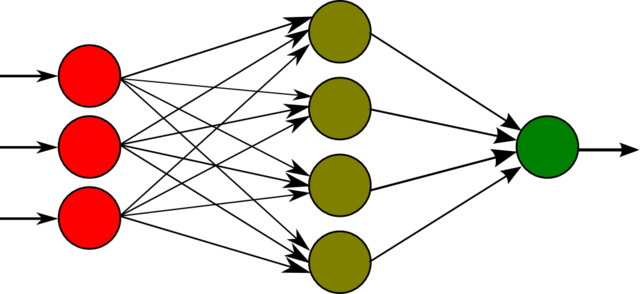
\includegraphics[scale=0.3]{images/single_layer_mlp_example}
  \end{figure}
  \FloatBarrier
  
  The nodes in a MLP are called neurons because MLPs were developed to model the workings of biological neurons in the
  brain. Each of the neurons in an MLP has an activation function. This function maps the weighted inputs to the output of
  each neuron. The activation function used is nonlinear and models the frequency of action potentials (this is what happens
  in the brain). The activation function used is typically either $y(v_{i}) = tanh(v_{i})$ or $y(v_{i}) = (1 + e^{-v_{i}})^{-1}$.
  Note that both of these functions are sigmoids (S-shaped curves).
  
  In this project, the MLP is parameterized by a set of weight matrices, $W_{i,j}$, and bias vectors, $b_{i}$. The weight
  matrices correspond to the weights of the connections between the nodes in layer $i$ to the nodes in layer $j$. Similarly,
  the bias vector $b_{i}$, defines any biases towards certain nodes in layer $i$.
  
  In order for a MLP to be an effective tool, the transformation $\Phi$ must be learned. This amounts to determining the
  appropriate bias and weight values. The transformation can be formally expressed as: \\
  \vspace{1mm}
  \hspace{7mm}$\Phi(x) = s(b_{i} + W_{i}x)$ \\
  In this formula $x$ is the input to layer $i$, $b$ is the bias vector, $W$ is the weight matrix and $s$ is the activation
  function.
  
  Learning the set of required parameters $\Theta$ is done using a gradient descent approach similar to that used in the
  logistic regression implementation. The gradients, $\frac{\partial \ell}{\partial \Theta}$, are obtained using the
  backpropogation algorithm.
  
  To use an MLP for classification of input, logistic regression can be used to determine the output. When this is the case,
  the output of an MLP can be formally described as: \\
  \vspace{1mm}
  \hspace{7mm}$o(x) = softmax(b_{n} + W_{n} \Phi(x))$ \\
  Where $n$ is the number of layers in the MLP.
  
  \subsubsection{Implementation}
  
  The implementation of a MLP was done in Python using the Theano library. Below is shown the code for the class that
  represents the hidden layer of the MLP. This layer is connected to an instance of the\textit{LogisticRegression} classifier.
  \lstinputlisting[language=Python, firstline=9, lastline=39]{../src/multilayer_perceptron.py}  
  
  \subsubsection{Results and Analysis} 

\subsection{Convolutional Neural Network}
  \subsubsection{Technique Overview}
  
  A Convolutional Neural Network (CNN) is a variant of the previously seen Multilayer Perceptron. CNNs are inspired by the
  structure of the visual cortex and its complex arrangement of cells.
  
  The visual cortex has been shown to be comprised of cells that are sensitive to small sub-regions of the visual-field. These
  sub-regions can be tiled to cover the entire visual field and are called receptive fields. These cells act as local filters
  over the input space and result in an exploitation of the spatial local correlation that occurs in natural images.
  
  Convolutional Neural Networks were designed to mirror the functionality of the visual cortex. They do this by enforcing a
  local connectivity pattern between neurons of adjacent layers to exploit spatial local correlation as well as using
  convolution of the input with a linear filter to repeatedly apply a function across sub-regions of the entire input.
  
  There are a number of CNNs modeled after the visual cortex. The architecture followed in this project is for the LeNet CNN
  developed by Yann LeCun at NYU.
  
  CNNs enforce local connectivity by having the inputs to the nodes in a hidden layer $h$ be from a subset of units in layer
  $h-1$ that have spatially contiguous receptive fields. This results in each node being unresponsive to variations outside
  of its 'receptive field', ensuring the strongest response to a spatially local input pattern.
  
  Convolution is used in the creation of a feature map. A feature map is a set of replicated nodes (replicated by applying a
  filter $h_{i}$ across the visual field) that share the same parameterization. One of these feature maps is obtained by
  convolution of the input with a linear filter, adding a bias and applying a non-linear function. A feature map $h_{k}$ can
  be obtained by: \\
  \vspace{1mm}
  \hspace{7mm}$h_{i,j}^{k} = s((W_{k} \ast x)_{i,j} + b_{k})$ \\
  In the above formula, $\ast$ is the convolution operator, $W$ is the weight matrix from layer $k-1$ to $k$, $b$ is the bias
  vector at layer $k$ and $s$ is the non-linear function used.
  
  The definition of convolution on a 2D signal is: \\
  $o(m,n) = f(m,n) \ast g(m,n) = \sum_{u=-\infty}^{\infty} \sum_{v=-\infty}^{\infty} f(u,v)g(m - u,n - v)$
  
  The implementation of a CNN, typically has each hidden layer composed of multiple feature maps to form a richer
  representation of the data. In this case, the connections, and weights, between two layers $m-1$ and $m$ are from each
  pixel of the $k$th feature map in layer $m$ to the pixel at coordinates $(i,j)$ of the $i$th feature map of layer $m-1$.
  The weights are then $W_{i,j}^{k,l}$. An example of a convolutional layer can be seen below: \\
  \FloatBarrier
  \begin{figure}[h]
    \caption{Convolutional Layer Example}
    \centering
    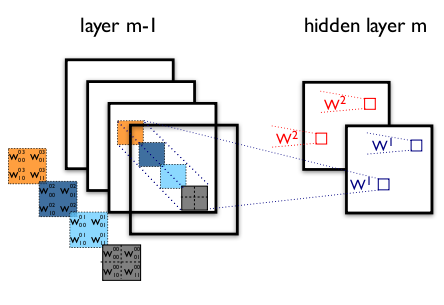
\includegraphics[scale=0.5]{images/conv_layer_cnn_example}
  \end{figure}
  \FloatBarrier
  
  In addition to a convolutional layer, CNNs also employ a form of non-linear down-sampling called \textbf{max pooling}.
  Max-pooling partitions an input into a set of non-overlapping rectangles and outputs the maximum value for each sub region.
  This step serves to reduce the computation required in upper layers of the CNN by eliminating non-maximal values as well as
  providing additional robustness to position.
  
  The CNN constructed for this project involves two convolutional layers, two max-pooling layers and one fully-connected
  hidden-layer (like that in an MLP) used for classification. An example of the architecture is: \\
  \FloatBarrier
  \begin{figure}[h]
    \caption{Convolutional Neural Network Example for MNIST dataset}
    \centering
    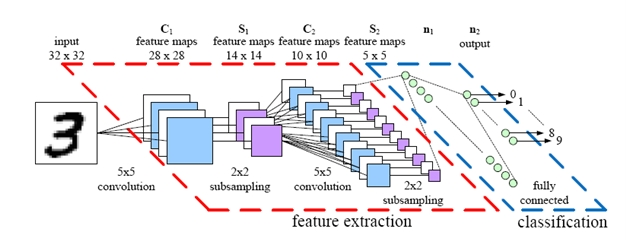
\includegraphics[scale=0.65]{images/architecture_cnn_example}
  \end{figure}
  \FloatBarrier
  
  \subsubsection{Implementation}
  
  The Convolutional Neural Network used in this project was written in Python using the Theano library. Below is the source
  code for the Convolutional and Max-Pooling layers of a CNN:
  \lstinputlisting[language=Python, firstline=8, lastline=47]{../src/convolutional_network.py}
  \vspace{3mm}
  The CNN is comprised of four layers:
  \begin{itemize}
    \item Two \textbf{Convolution and Max-Pooling layers}
    \item One \textbf{Fully-connected Hidden Layer}
    \item One \textbf{Logistic Regression Classifier}
  \end{itemize}
  Below is the source code for a complete CNN implementation:
  \lstinputlisting[language=Python, firstline=48, lastline=221]{../src/convolutional_network.py}
  
  \subsubsection{Results and Analysis}
  
\newpage
\section{Application of Techniques}

This section will outline the usage of the techniques described above.

\subsection{Goal}

The desired outcome of this project is to gain insight into the similarity of sets of images. To this end, the project
looks to examine the analysis of a set of like-images resulting in a description of the unique 'features' of that set that
can then be used to examine similarity of images with respect to the discovered features. This task is closely intertwined
with current computer vision techniques used in the identification of images and so another intended result was an exploration
of the techniques currently used for image identification tasks.
  
\subsection{Approach}

This section will outline the usage of the different techniques outlined in the previous section. It will also examine the
process used to attempt to achieve the proposed goal.

As described in the previous section, the techniques used in this project are as the follows:
\begin{enumerate}
  \item Principal Components Analysis
  \item Logistic Regression Classifier
  \item Convolutional Neural Network (incorporates Multilayer Perceptron)
\end{enumerate}

What follows is an outline of the how the above techniques were used to extract the features of a given dataset $D$:
\begin{itemize}
  \item \textbf{Whitening the Data} \\
        Principal Components Analysis was used to apply the Whitening Transformation to the input data. This results in
        pre-processing the data to be uncorrelated with a variance of 1. This boosts the areas of high contrast in the image
        and increases the accuracy of the analysis techniques

  \item \textbf{Training the Convolutional Neural Network}
  		The dataset $D$ is used to train a Convolutional Neural Network. This process causes the parameters of the CNN model
  		to be unique to the given dataset. In other words, what is obtained by training a CNN, is a unique set of parameters
  		$\Theta$ that corresponds to the weights and biases of the different layers.
  		
  \item \textbf{Verify of Accuracy of the CNN Classification}
  		After a Convolutional Neural Network has been trained, verification of the results obtained is necessary to see if the
  		parameters yield a satisfactory result in labeling new data. 
\end{itemize}

The above process outlines the steps necessary to take a dataset $D$ and obtain a unique description of the dataset in the
form of a set of weights and bias vectors for the different layers of the CNN. For this approach to work, the dataset must be
images that have been identified to be alike. In testing this process, the custom dataset outlined in section 2.3 was used.
  
\subsection{Results}

\section{Technical Challenges and Comments}
\subsection{Python Libraries}

\section{Project Criterion Overview}

\end{document}
